% Options for packages loaded elsewhere
\PassOptionsToPackage{unicode}{hyperref}
\PassOptionsToPackage{hyphens}{url}
%
\documentclass[
]{book}
\usepackage{amsmath,amssymb}
\usepackage{lmodern}
\usepackage{ifxetex,ifluatex}
\ifnum 0\ifxetex 1\fi\ifluatex 1\fi=0 % if pdftex
  \usepackage[T1]{fontenc}
  \usepackage[utf8]{inputenc}
  \usepackage{textcomp} % provide euro and other symbols
\else % if luatex or xetex
  \usepackage{unicode-math}
  \defaultfontfeatures{Scale=MatchLowercase}
  \defaultfontfeatures[\rmfamily]{Ligatures=TeX,Scale=1}
\fi
% Use upquote if available, for straight quotes in verbatim environments
\IfFileExists{upquote.sty}{\usepackage{upquote}}{}
\IfFileExists{microtype.sty}{% use microtype if available
  \usepackage[]{microtype}
  \UseMicrotypeSet[protrusion]{basicmath} % disable protrusion for tt fonts
}{}
\makeatletter
\@ifundefined{KOMAClassName}{% if non-KOMA class
  \IfFileExists{parskip.sty}{%
    \usepackage{parskip}
  }{% else
    \setlength{\parindent}{0pt}
    \setlength{\parskip}{6pt plus 2pt minus 1pt}}
}{% if KOMA class
  \KOMAoptions{parskip=half}}
\makeatother
\usepackage{xcolor}
\IfFileExists{xurl.sty}{\usepackage{xurl}}{} % add URL line breaks if available
\IfFileExists{bookmark.sty}{\usepackage{bookmark}}{\usepackage{hyperref}}
\hypersetup{
  pdftitle={PBWG Interactive Report},
  pdfauthor={PBWG Members},
  hidelinks,
  pdfcreator={LaTeX via pandoc}}
\urlstyle{same} % disable monospaced font for URLs
\usepackage{longtable,booktabs,array}
\usepackage{calc} % for calculating minipage widths
% Correct order of tables after \paragraph or \subparagraph
\usepackage{etoolbox}
\makeatletter
\patchcmd\longtable{\par}{\if@noskipsec\mbox{}\fi\par}{}{}
\makeatother
% Allow footnotes in longtable head/foot
\IfFileExists{footnotehyper.sty}{\usepackage{footnotehyper}}{\usepackage{footnote}}
\makesavenoteenv{longtable}
\usepackage{graphicx}
\makeatletter
\def\maxwidth{\ifdim\Gin@nat@width>\linewidth\linewidth\else\Gin@nat@width\fi}
\def\maxheight{\ifdim\Gin@nat@height>\textheight\textheight\else\Gin@nat@height\fi}
\makeatother
% Scale images if necessary, so that they will not overflow the page
% margins by default, and it is still possible to overwrite the defaults
% using explicit options in \includegraphics[width, height, ...]{}
\setkeys{Gin}{width=\maxwidth,height=\maxheight,keepaspectratio}
% Set default figure placement to htbp
\makeatletter
\def\fps@figure{htbp}
\makeatother
\setlength{\emergencystretch}{3em} % prevent overfull lines
\providecommand{\tightlist}{%
  \setlength{\itemsep}{0pt}\setlength{\parskip}{0pt}}
\setcounter{secnumdepth}{5}
\usepackage{booktabs}
\usepackage{amsthm}
\makeatletter
\def\thm@space@setup{%
  \thm@preskip=8pt plus 2pt minus 4pt
  \thm@postskip=\thm@preskip
}
\makeatother
\ifluatex
  \usepackage{selnolig}  % disable illegal ligatures
\fi
\usepackage[]{natbib}
\bibliographystyle{apalike}

\title{PBWG Interactive Report}
\author{PBWG Members}
\date{2021-04-27}

\begin{document}
\maketitle

{
\setcounter{tocdepth}{1}
\tableofcontents
}
\hypertarget{front-matters}{%
\chapter*{Front Matters}\label{front-matters}}
\addcontentsline{toc}{chapter}{Front Matters}

The Performance Benchmarking Working Group aims to foster the understanding of the ICAO Global Air Navigation Plan (GANP) key performance indicators and jointly works on establishing commonly agreed definitions and algorithms in support of the GANP.
This report reflects a set of air traffic measures addressing the current COVID/post-COVID developments.

PBWG Members are

\begin{itemize}
\tightlist
\item
  Brazil, DECEA
\item
  Europe, EUROCONTROL
\item
  Japan, JCAB
\item
  Singapore, CAAS
\item
  Thailand, AEROTHAI
\item
  United States of America, FAA
\end{itemize}

\hypertarget{introduction}{%
\chapter{Introduction}\label{introduction}}

The present briefing aims to provide a comparison of the COVID-19 impacts on aviation in different parts of the world. The regions covered herein are Brazil, Europe, Japan, Thailand, Singapore and the United States.

\hypertarget{scope}{%
\chapter{Scope}\label{scope}}

The following airports are covered by this briefing:

\hypertarget{brazil-airports}{%
\section{Brazil airports}\label{brazil-airports}}

SBBR, SBCF, SBCT, SBFL, SBGL, SBGR, SBKP, SBPA, SBRF, SBRJ, SBSP, and SBSV

\hypertarget{europe-airports}{%
\section{Europe airports}\label{europe-airports}}

EDDF, EDDM, EGLL, EHAM, LEMD, LFPG, LIRF, and LSZH

\hypertarget{japan-airports}{%
\section{Japan airports}\label{japan-airports}}

TBD

\hypertarget{thailand-airports}{%
\section{Thailand airports}\label{thailand-airports}}

VTBD, VTBS, VTCC, and VTSP

\hypertarget{singapore-airports}{%
\section{Singapore airports}\label{singapore-airports}}

WSSS

\hypertarget{usa-airports}{%
\section{USA airports}\label{usa-airports}}

TBD

\hypertarget{overview-comparison}{%
\chapter{Overview comparison}\label{overview-comparison}}

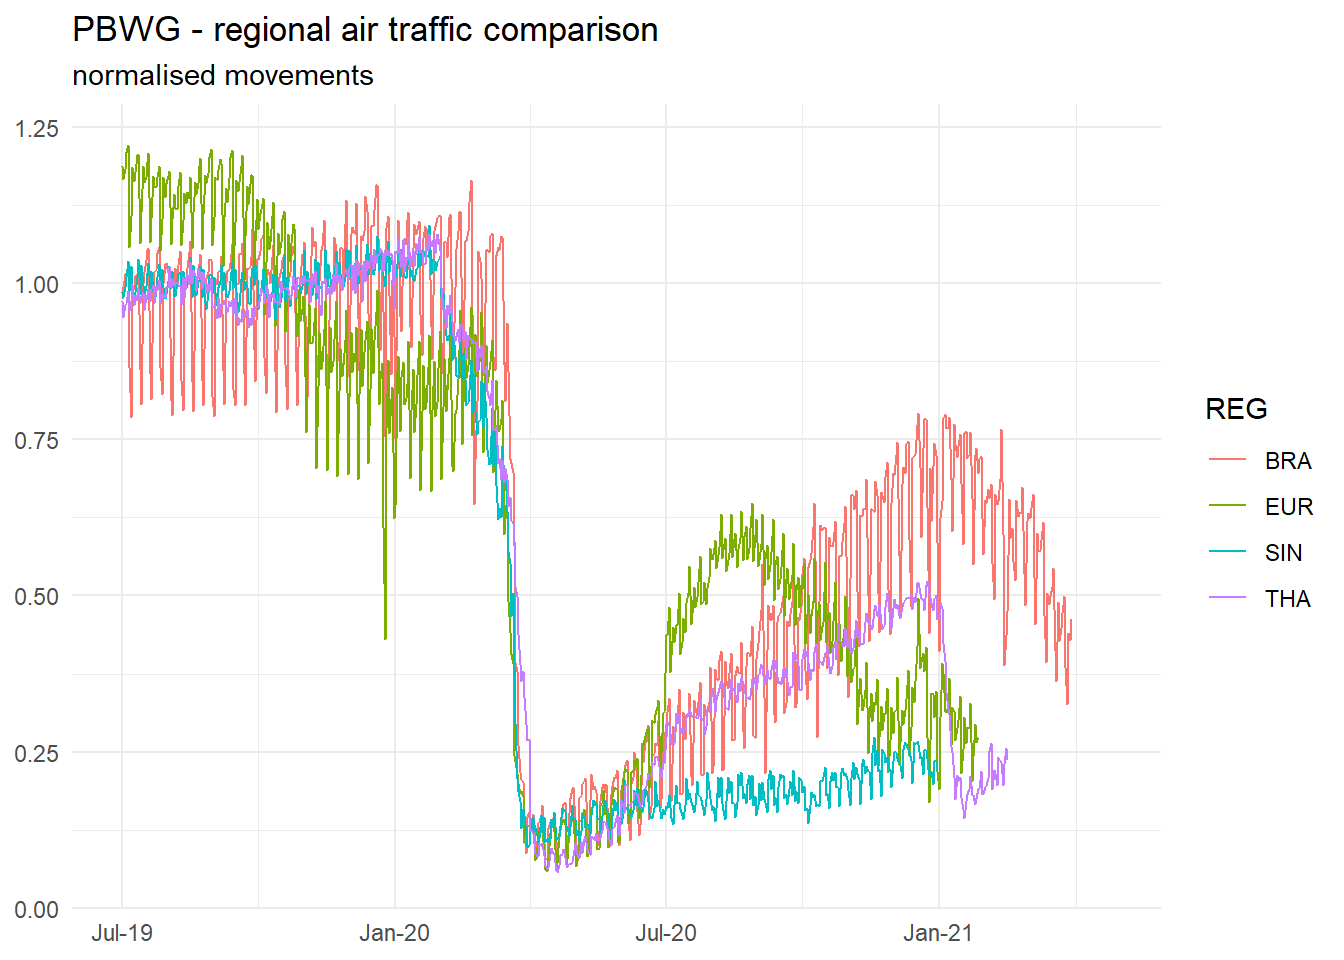
\includegraphics{bookdown-demo_files/figure-latex/unnamed-chunk-4-1.pdf}

\hypertarget{overflights}{%
\section{Overflights}\label{overflights}}

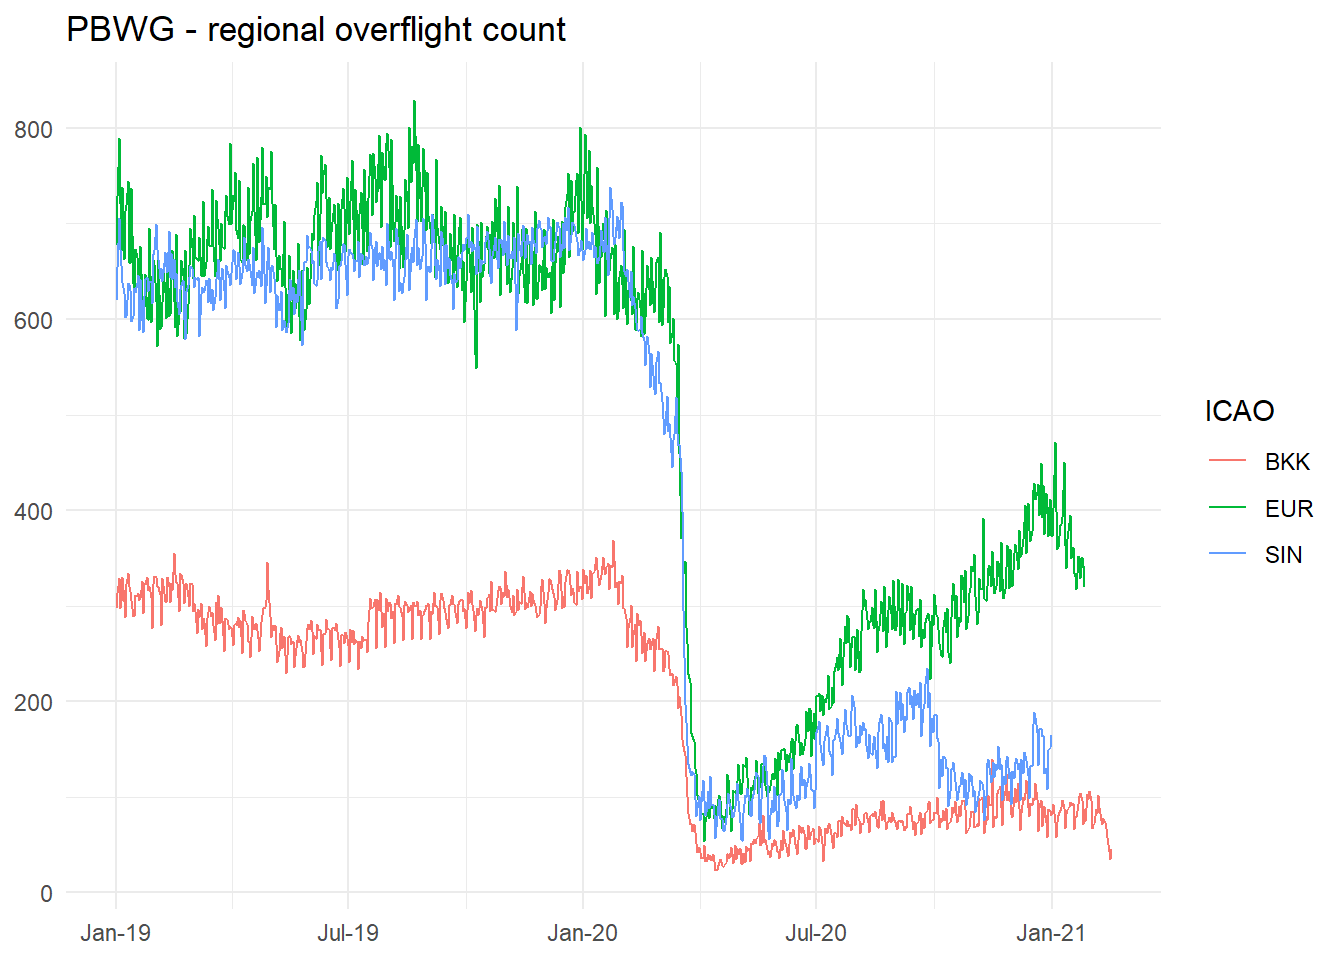
\includegraphics{bookdown-demo_files/figure-latex/unnamed-chunk-5-1.pdf}

\hypertarget{international-traffic}{%
\section{International traffic}\label{international-traffic}}

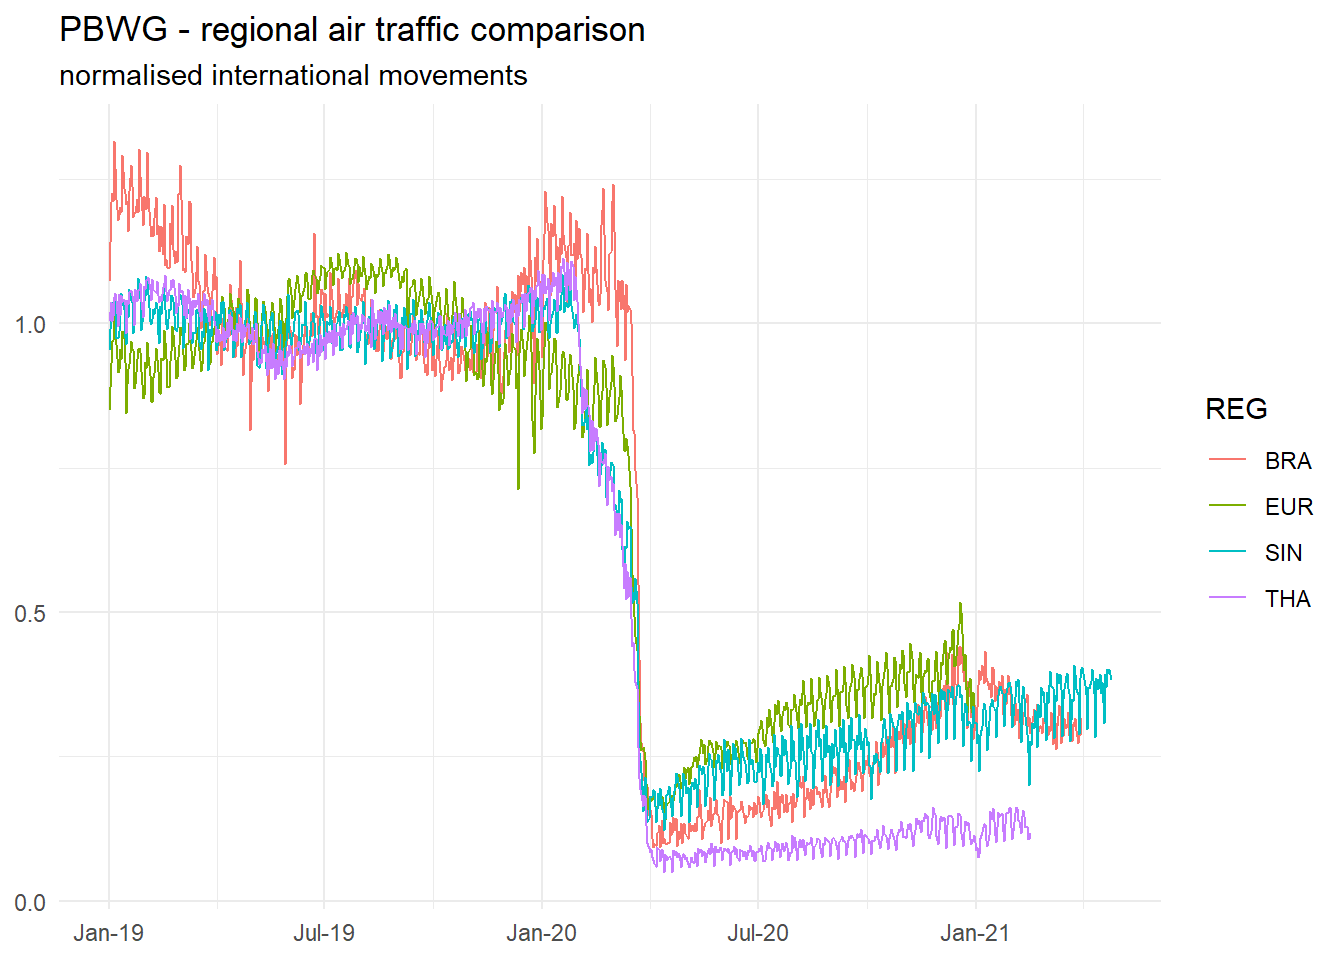
\includegraphics{bookdown-demo_files/figure-latex/unnamed-chunk-6-1.pdf}

\hypertarget{region-level-breakdown}{%
\chapter{Region level breakdown}\label{region-level-breakdown}}

\hypertarget{brazil}{%
\section{Brazil}\label{brazil}}

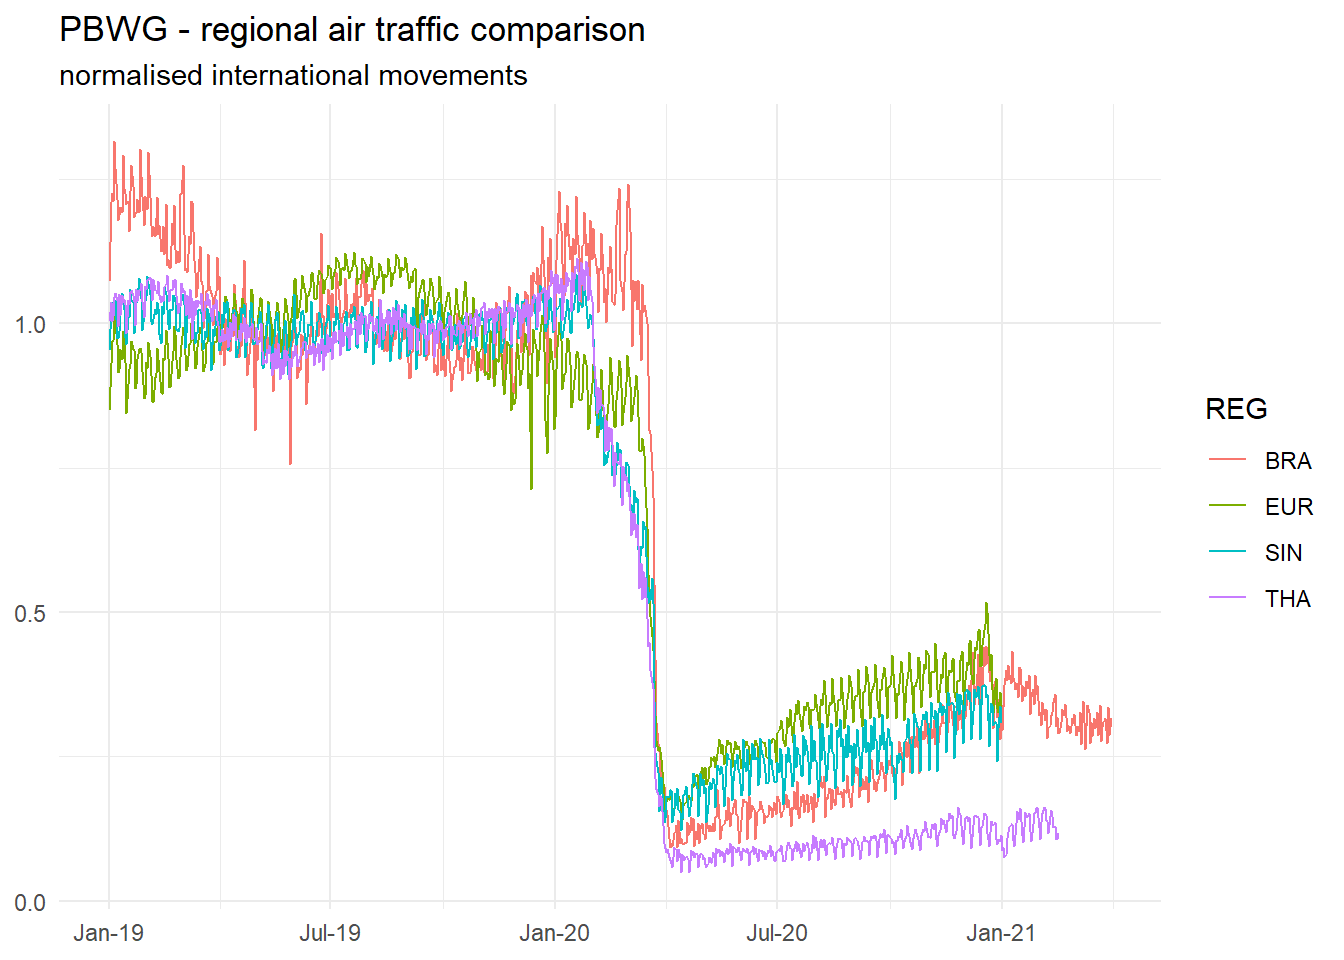
\includegraphics{bookdown-demo_files/figure-latex/unnamed-chunk-7-1.pdf}

\hypertarget{europe}{%
\section{Europe}\label{europe}}

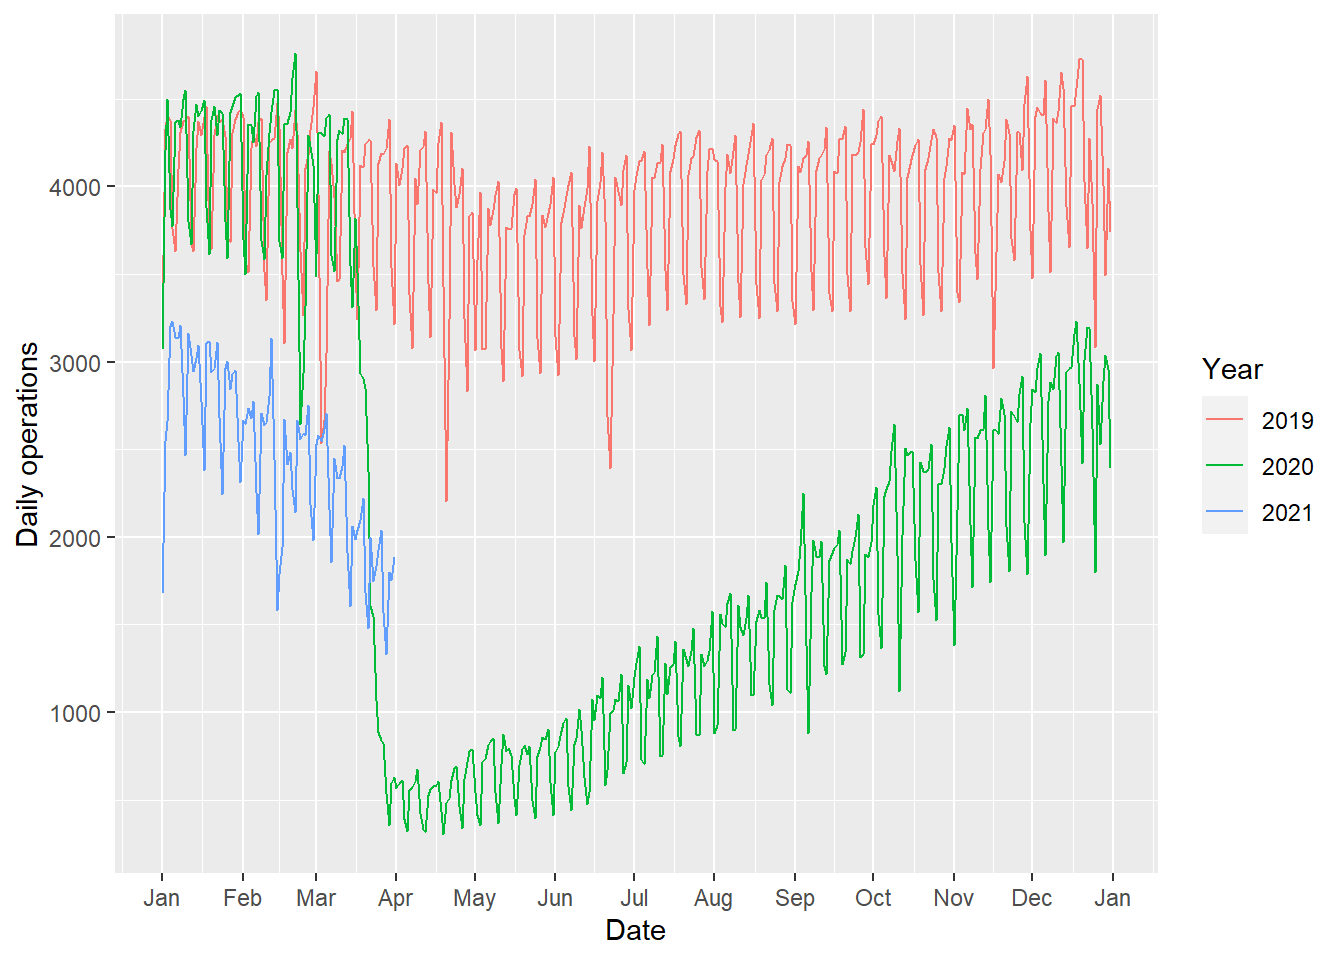
\includegraphics{bookdown-demo_files/figure-latex/unnamed-chunk-8-1.pdf}

\hypertarget{thailand}{%
\section{Thailand}\label{thailand}}

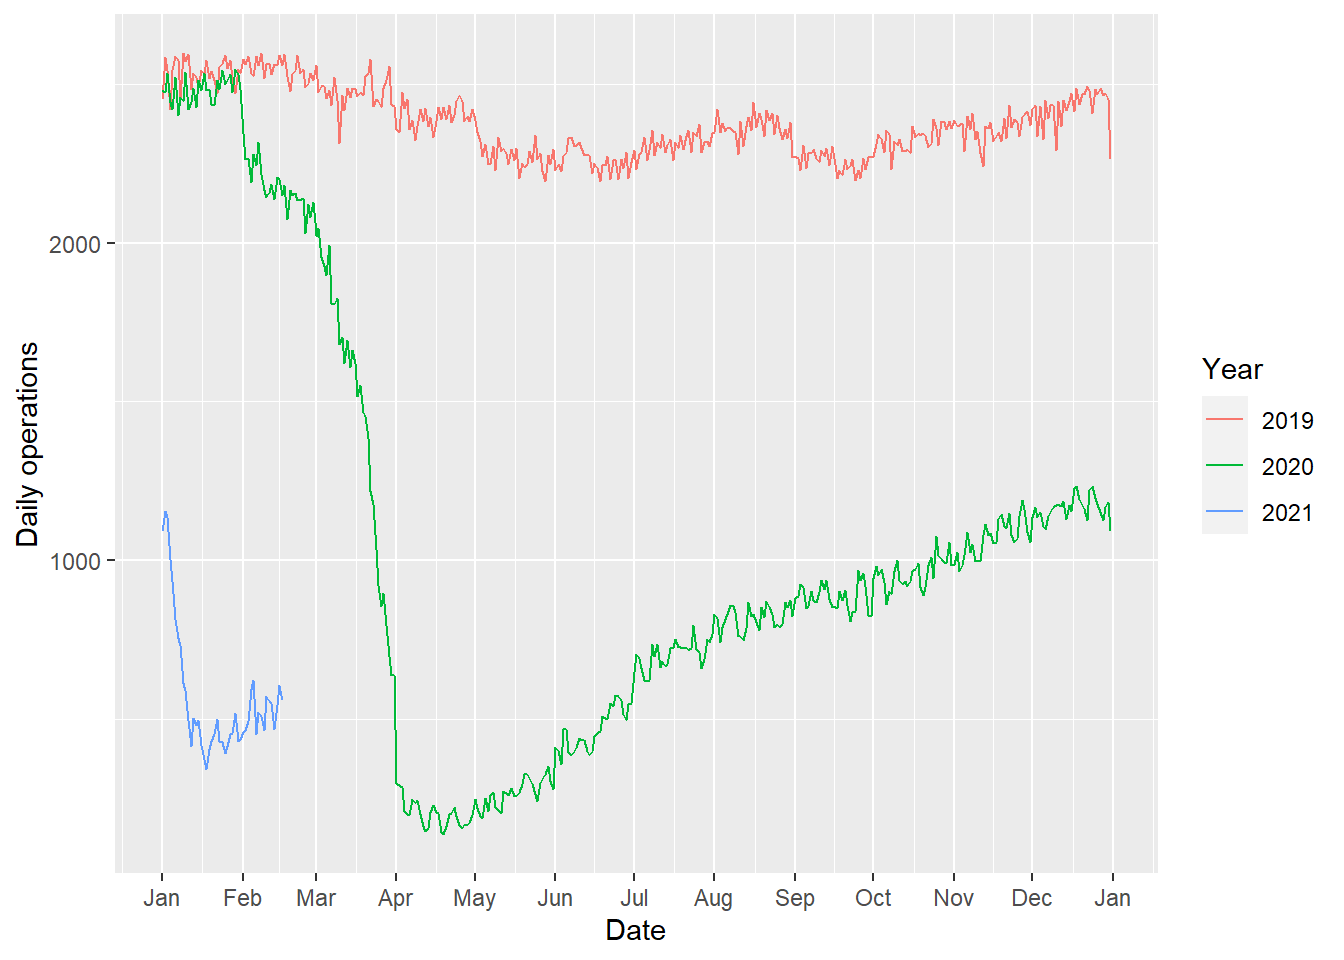
\includegraphics{bookdown-demo_files/figure-latex/unnamed-chunk-9-1.pdf}

\hypertarget{singapore}{%
\section{Singapore}\label{singapore}}

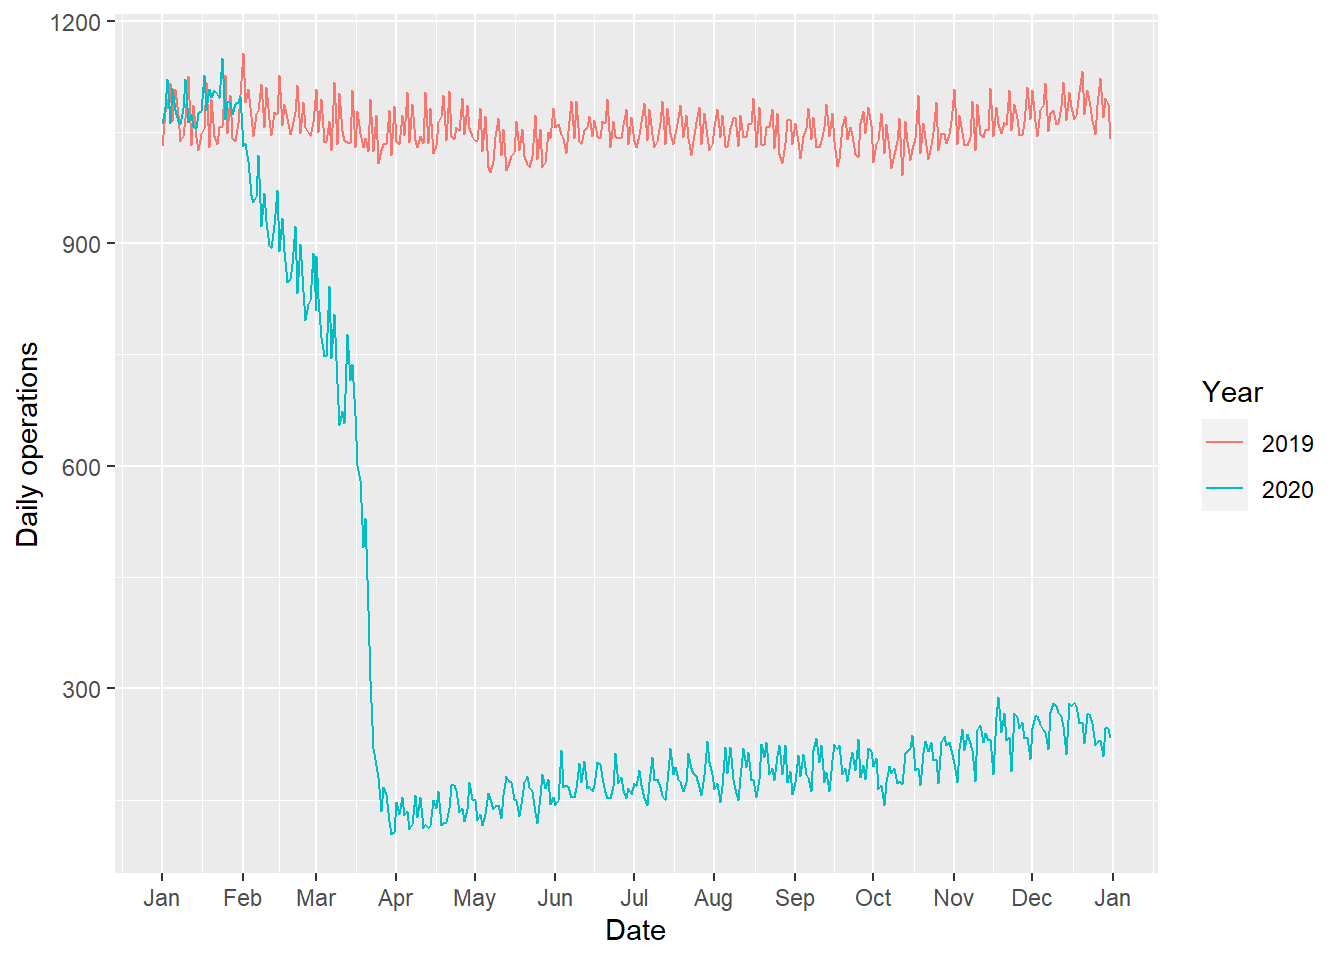
\includegraphics{bookdown-demo_files/figure-latex/unnamed-chunk-10-1.pdf}

\hypertarget{airport-level-breakdown}{%
\chapter{Airport level breakdown}\label{airport-level-breakdown}}

In 2020, the coronavirus crisis represented very different impacts depending on the airport. Figure n below shows the drop of flight operations (departures and arrivals), in comparison to 2019, at the airports under study.
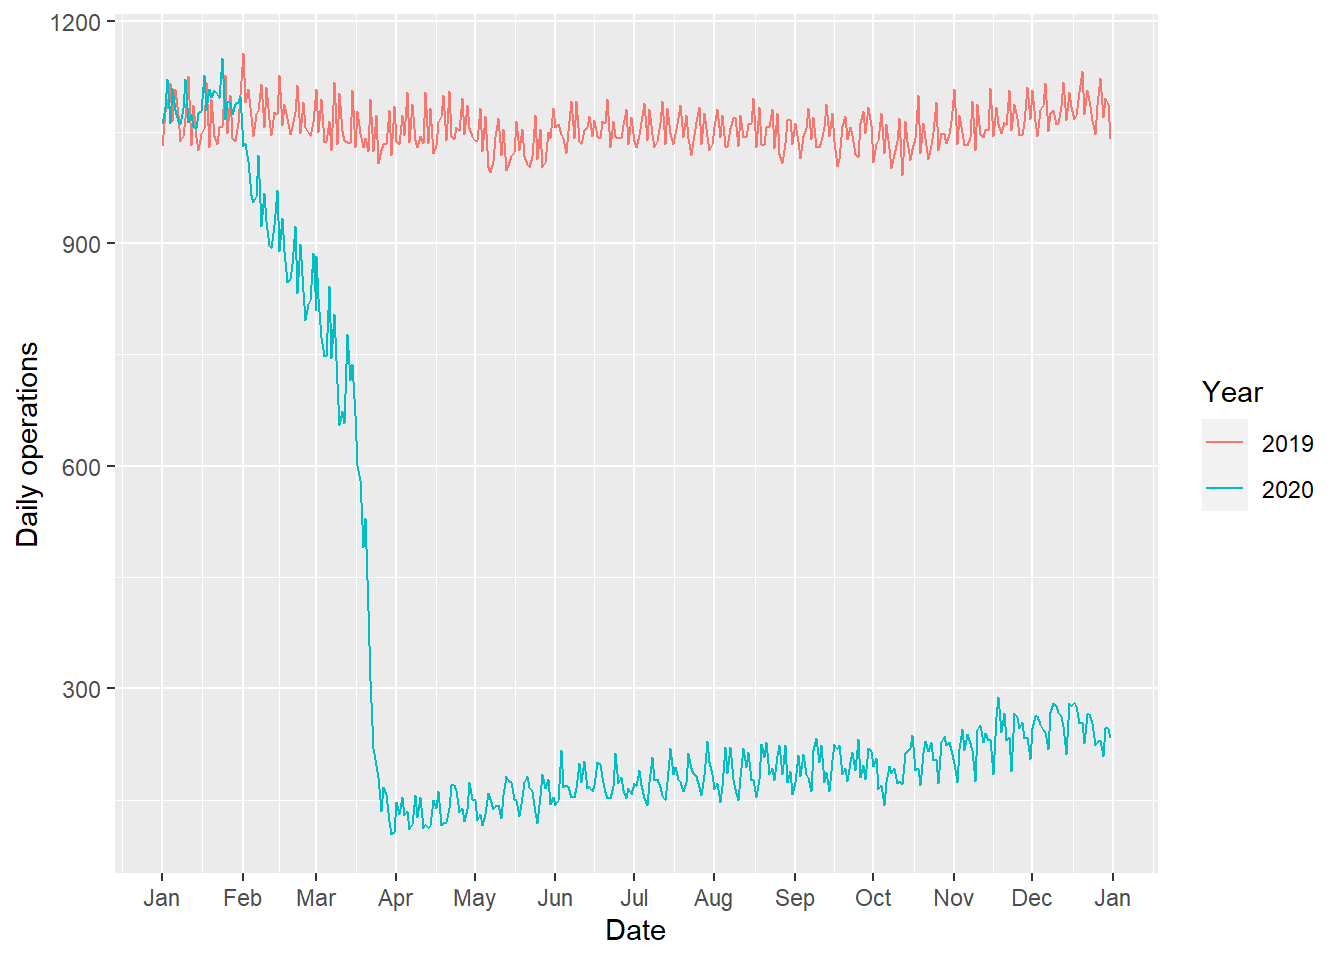
\includegraphics{bookdown-demo_files/figure-latex/unnamed-chunk-11-1.pdf}
All airports had decreases in their movements, ranging from -36\% to -67\%. In general, Singapore suffered the most, for the international travels were greatly affected. Brazilian airports had lower impacts than Europe. SBKP Campinas, for example, had -36\% - which is not so bad, giving the context. That happened probably due to a larger share of cargo aviation at that particular airport.

Except for Singapore, which has only one airport in the study, it is possible to look the different effects on individual airports within each region.

\hypertarget{brazil-airports-1}{%
\section{Brazil airports}\label{brazil-airports-1}}

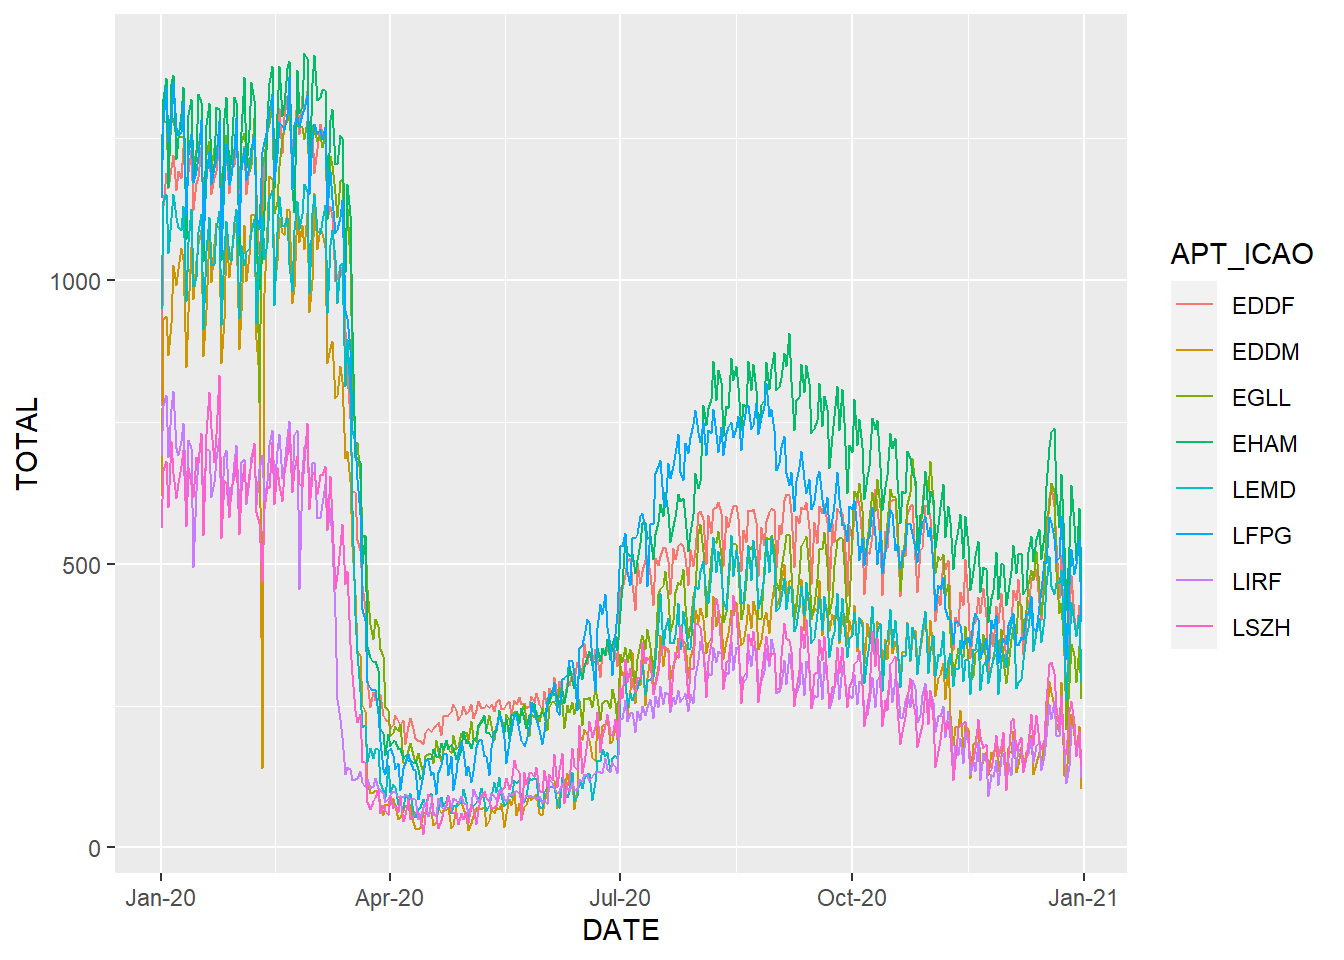
\includegraphics{bookdown-demo_files/figure-latex/unnamed-chunk-12-1.pdf} 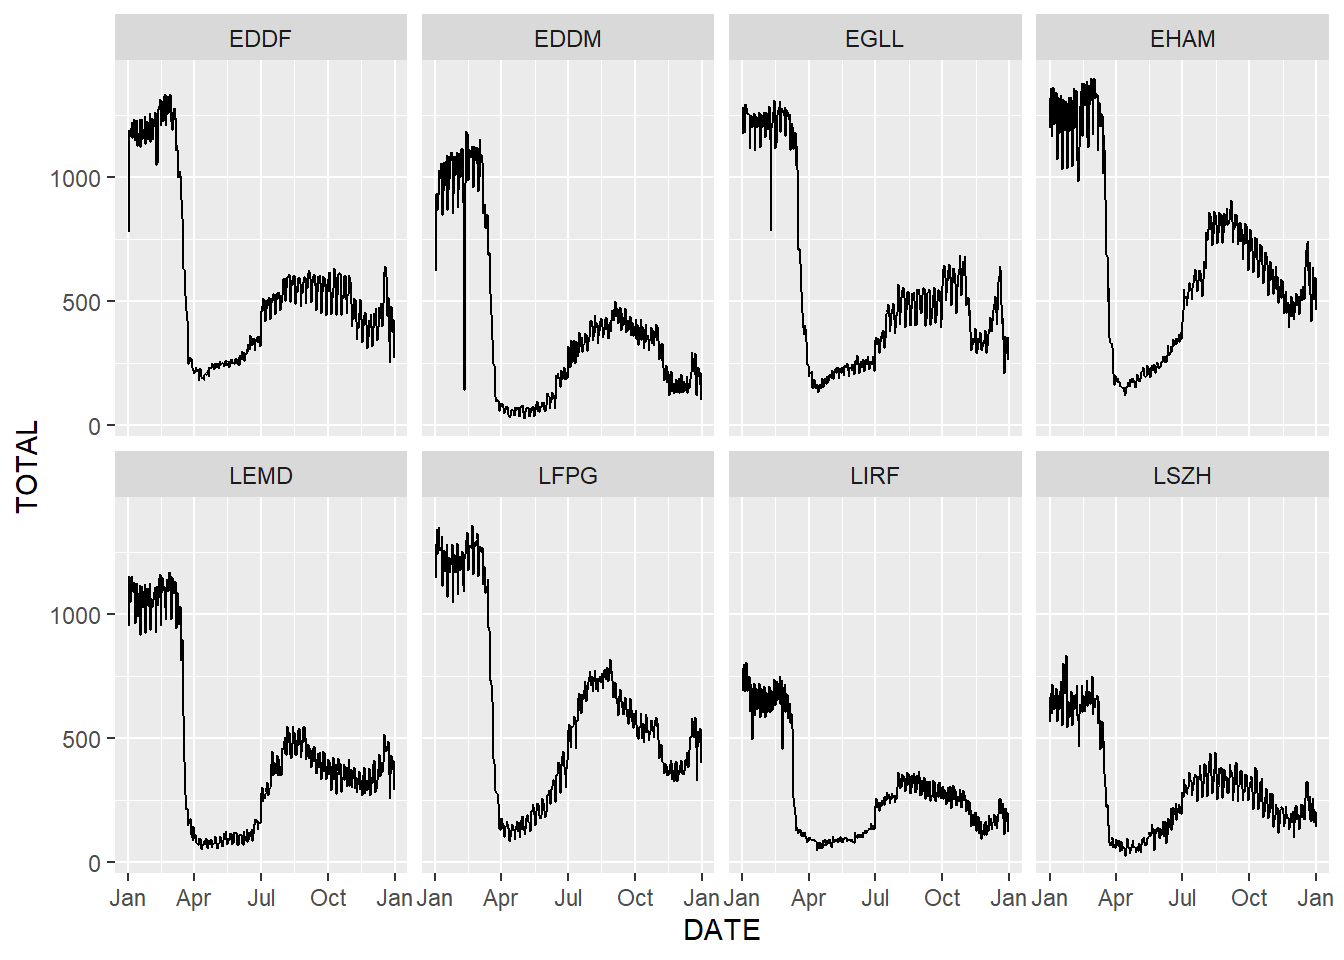
\includegraphics{bookdown-demo_files/figure-latex/unnamed-chunk-12-2.pdf}

\hypertarget{europe-airports-1}{%
\section{Europe airports}\label{europe-airports-1}}

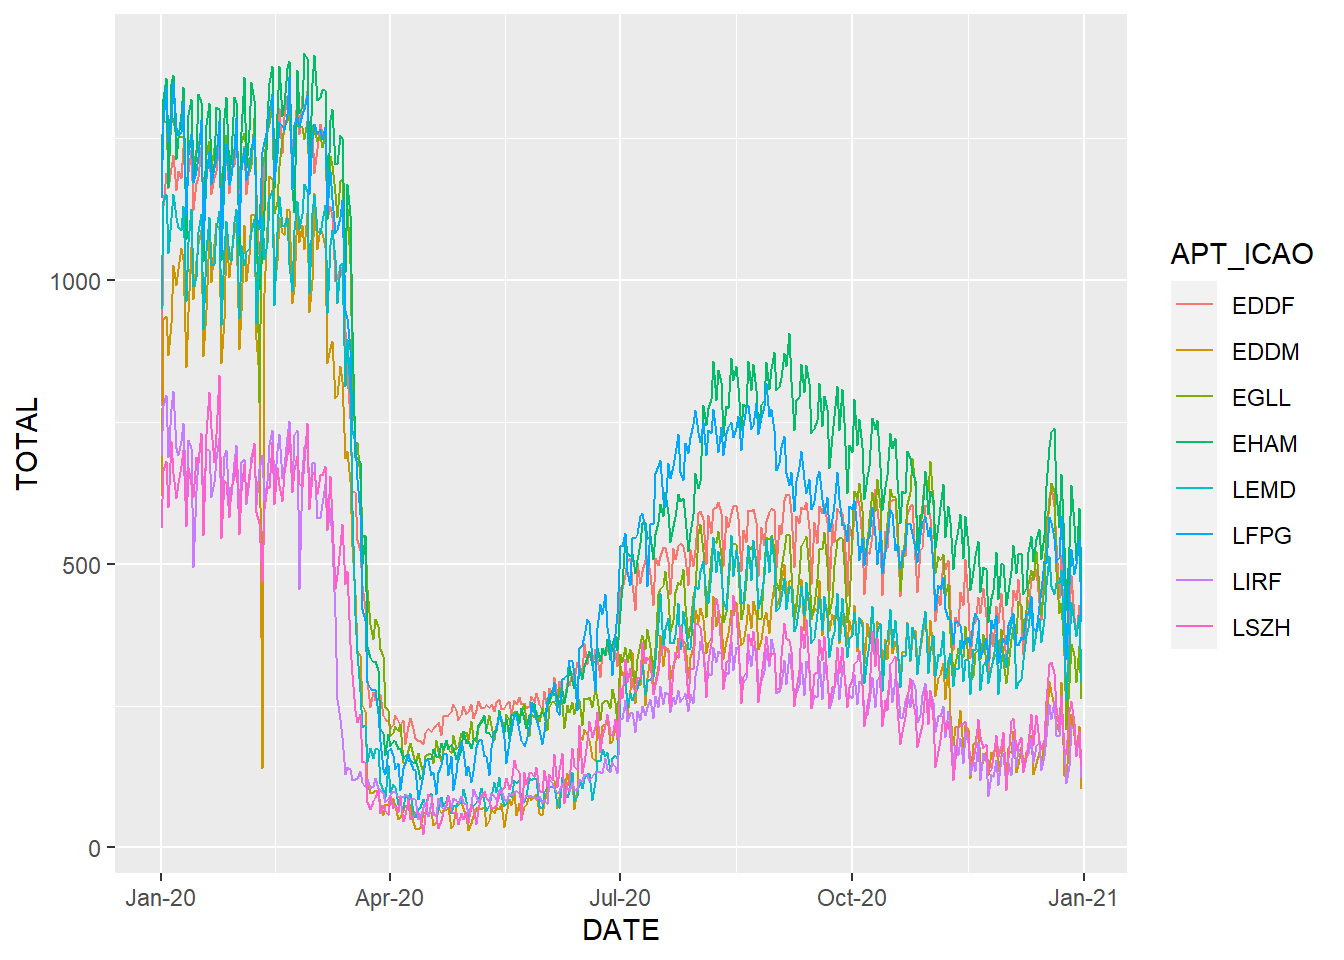
\includegraphics{bookdown-demo_files/figure-latex/unnamed-chunk-13-1.pdf} 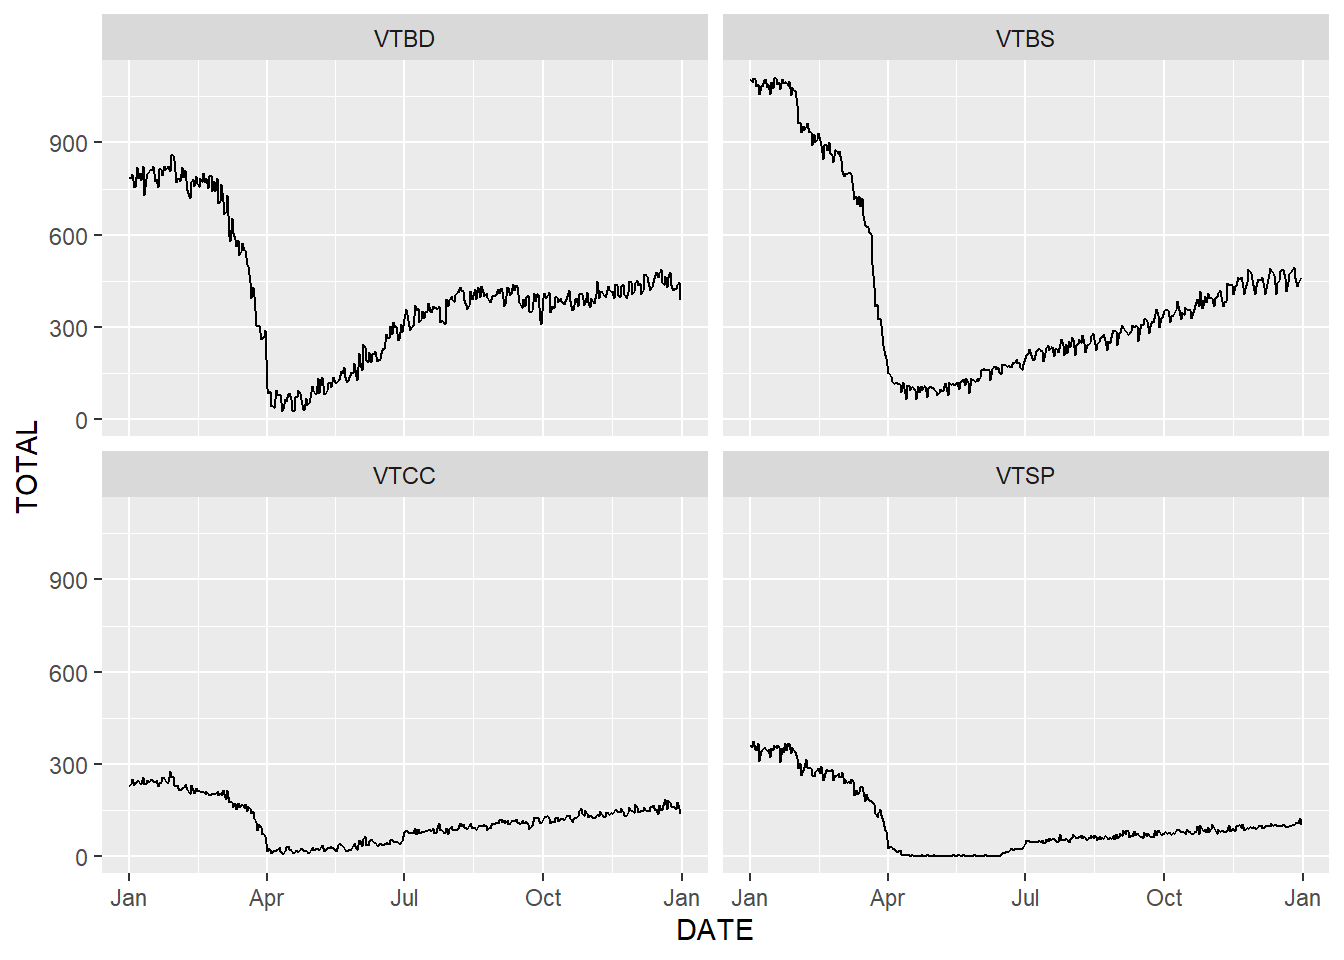
\includegraphics{bookdown-demo_files/figure-latex/unnamed-chunk-13-2.pdf}

\hypertarget{thailand-airports-1}{%
\section{Thailand airports}\label{thailand-airports-1}}

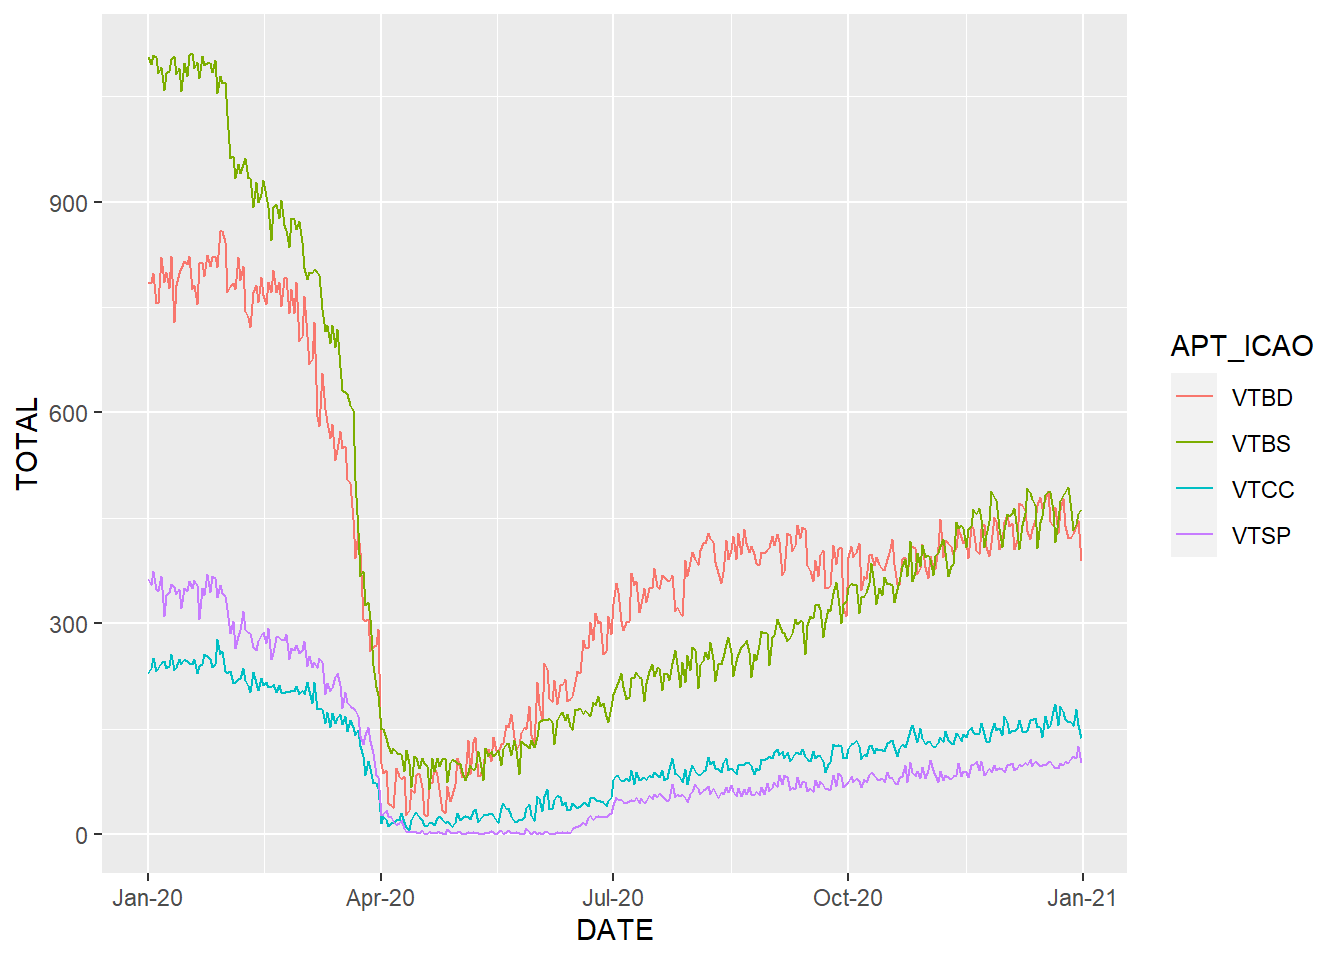
\includegraphics{bookdown-demo_files/figure-latex/unnamed-chunk-14-1.pdf} 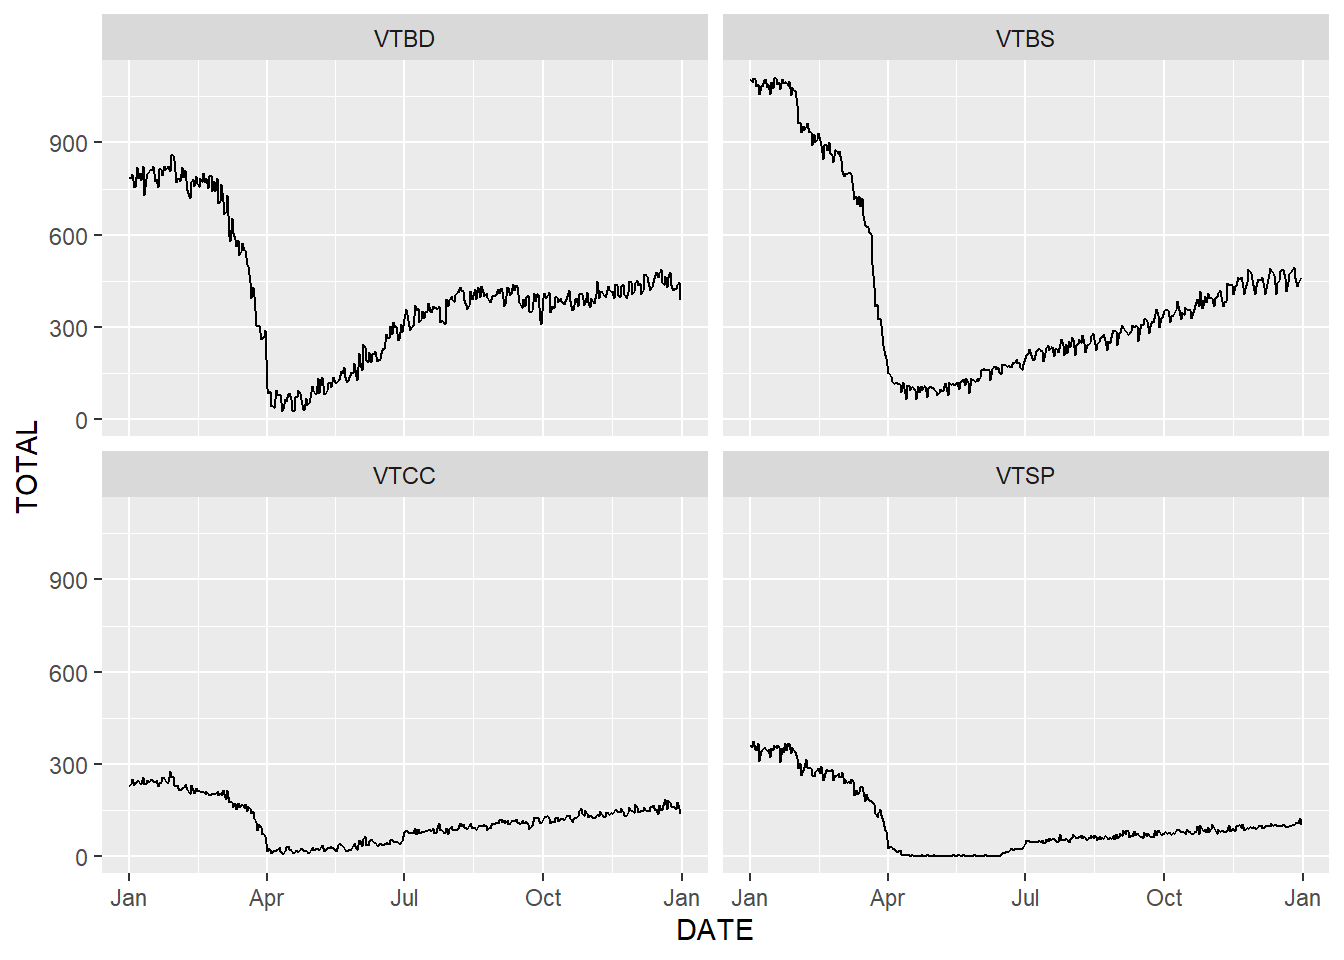
\includegraphics{bookdown-demo_files/figure-latex/unnamed-chunk-14-2.pdf}

\hypertarget{top-city-pairs}{%
\chapter{Top city pairs}\label{top-city-pairs}}

\hypertarget{brazil-routes}{%
\section{Brazil routes}\label{brazil-routes}}

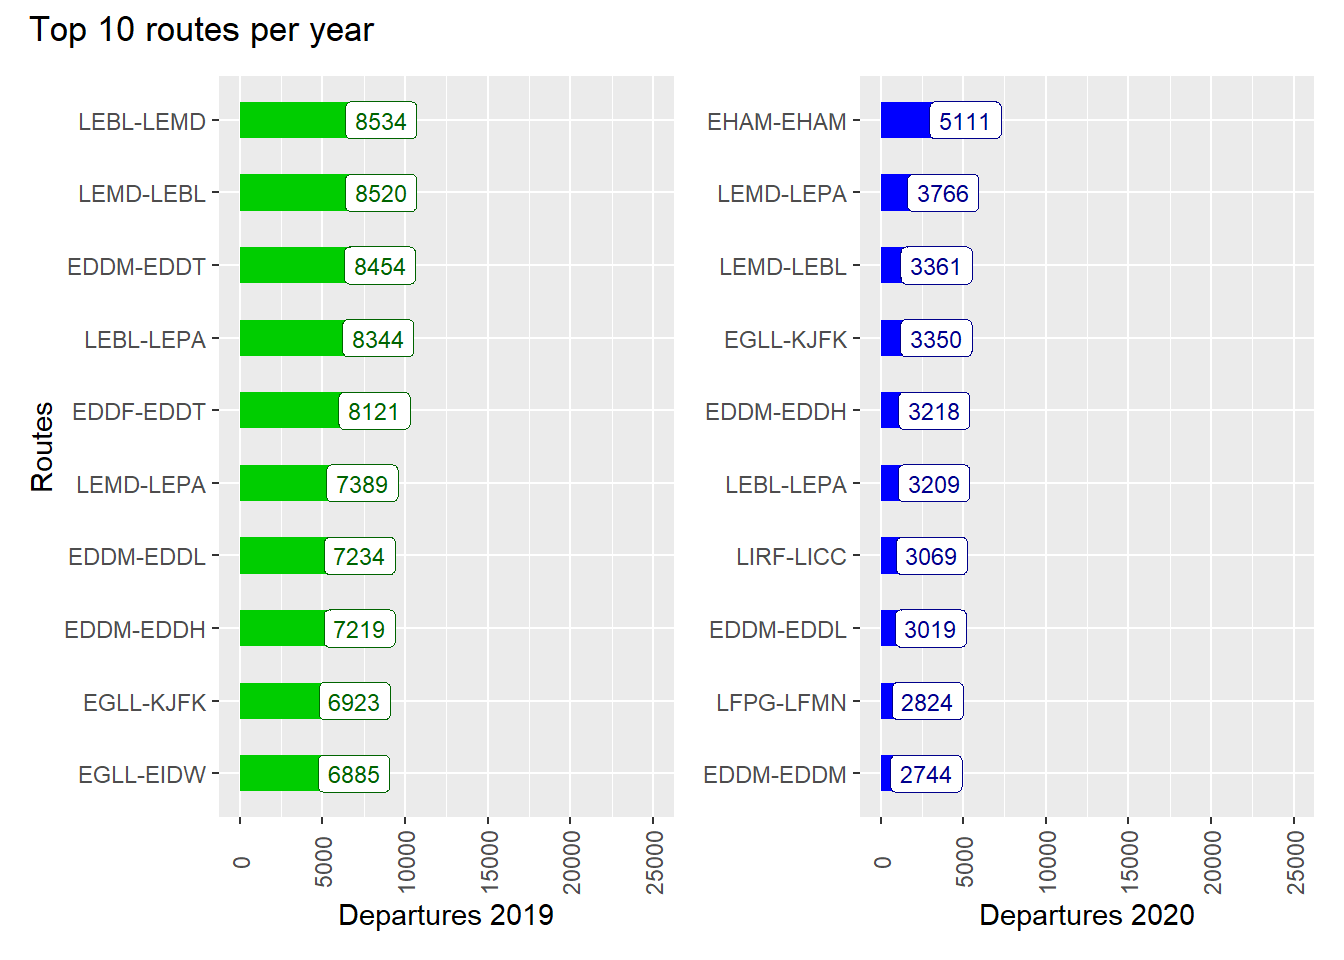
\includegraphics{bookdown-demo_files/figure-latex/unnamed-chunk-16-1.pdf}

\hypertarget{europe-routes}{%
\section{Europe routes}\label{europe-routes}}

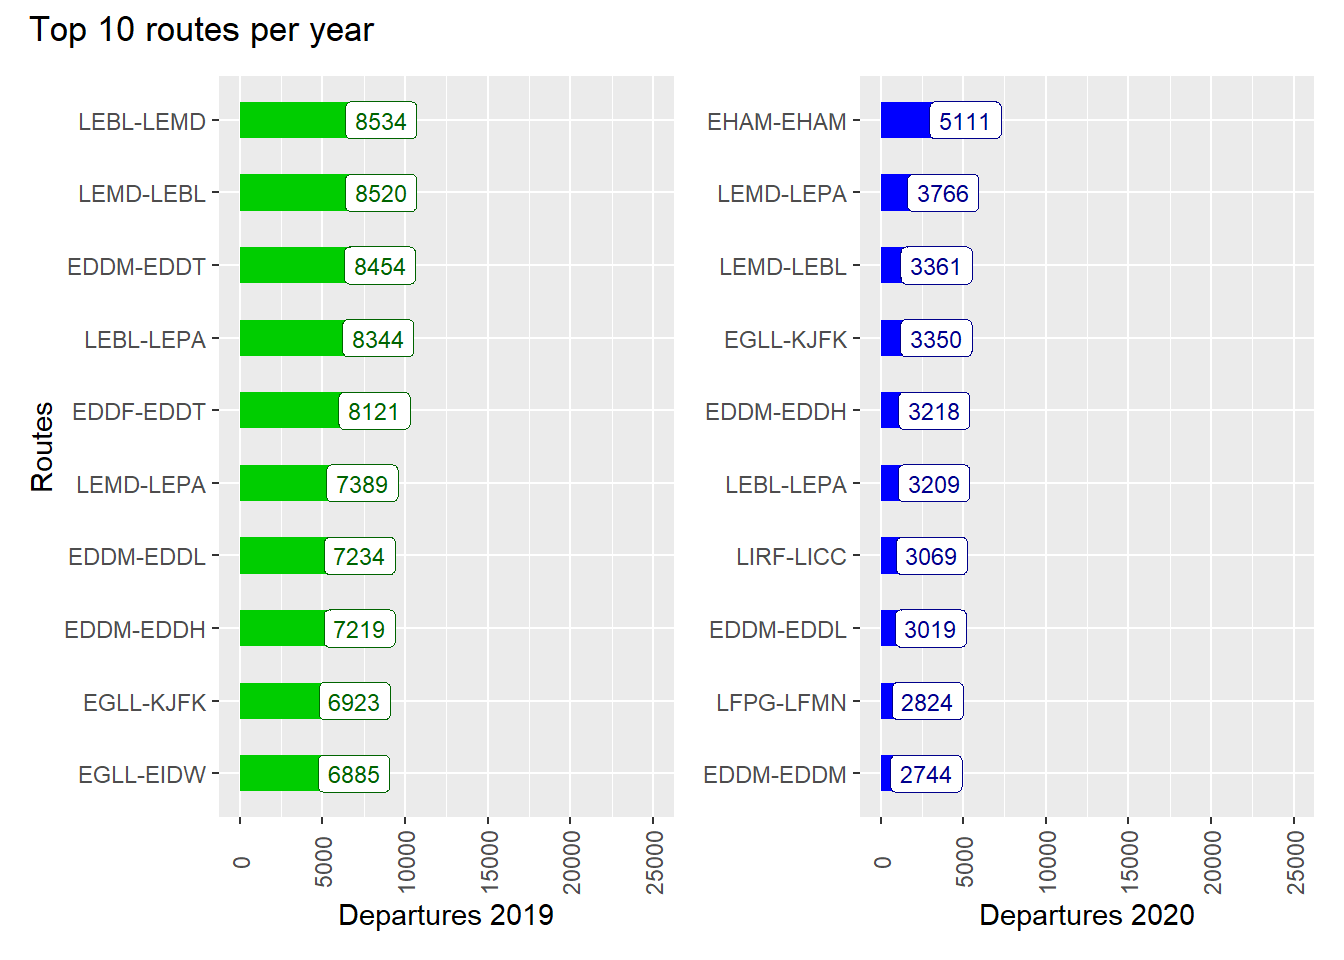
\includegraphics{bookdown-demo_files/figure-latex/unnamed-chunk-17-1.pdf}

  \bibliography{book.bib,packages.bib}

\end{document}
